\chapter{Results}
\label{ch:results}

This chapter reports every result obtained. Part A compares the reproduction with the RiskSEA paper table by table. Part B reports the tracing results of CryptoTrace on three cases, the comparison of strategies, the cost, and a walk through every screen of the application with its screenshot. Section~\ref{sec:improvements} states what was improved over the baseline and what was not.

\section*{Part A: Reproduction of RiskSEA}
\addcontentsline{toc}{section}{Part A: Reproduction of RiskSEA}

\section{Table II: Behavioural Features, node2vec, and Both}
\label{sec:t2}
Table~\ref{tab:t2} puts the paper's Table~II next to our two variants (all \NumLabeled{} labeled addresses). Table~\ref{tab:t2d} adds confidence intervals and control experiments.
\begin{table}[H]
\centering\footnotesize\singlespacing
\begin{tabular}{l ccc ccc ccc}
\toprule
 & \multicolumn{3}{c}{Paper} & \multicolumn{3}{c}{Ours, variant A} & \multicolumn{3}{c}{Ours, variant B}\\
\cmidrule(lr){2-4}\cmidrule(lr){5-7}\cmidrule(lr){8-10}
Features & P & R & F$_1$ & P & R & F$_1$ & P & R & F$_1$\\
\midrule
Behavioral features & 0.803 & 0.650 & 0.718 & 0.949 & 0.963 & 0.956 & 0.949 & 0.963 & 0.956\\
Node2vec embedding & 0.798 & 0.686 & 0.738 & 0.907 & 0.840 & 0.871 & 0.790 & 0.721 & 0.753\\
Node2vec + behavioral & 0.908 & 0.801 & 0.851 & 0.973 & 0.956 & 0.964 & 0.970 & 0.950 & 0.960\\
\bottomrule
\end{tabular}
\caption{Precision (P), recall (R) and F$_1$ at threshold 0.5. Paper values are from its Table~II. Variant A: labeled addresses are in the core; variant B: labeled addresses receive propagated embeddings only.}
\label{tab:t2}
\end{table}
\begin{table}[H]
\centering\scriptsize\singlespacing
\setlength{\tabcolsep}{3pt}\begin{tabular}{l r r ccc ccc}
\toprule
 & & & \multicolumn{3}{c}{F$_1$} & \multicolumn{3}{c}{PR-AUC}\\
\cmidrule(lr){4-6}\cmidrule(lr){7-9}
Variant & bad & good & behav. & n2v & both & behav. & n2v & both\\
\midrule
A: labeled in core & 481 & 4,080 & 0.956{\scriptsize$\pm$0.012} & 0.871{\scriptsize$\pm$0.018} & 0.964{\scriptsize$\pm$0.008} & 0.985{\scriptsize$\pm$0.009} & 0.939{\scriptsize$\pm$0.011} & 0.991{\scriptsize$\pm$0.006}\\
A, no miners & 481 & 127 & 0.982{\scriptsize$\pm$0.015} & 0.988{\scriptsize$\pm$0.004} & 0.987{\scriptsize$\pm$0.009} & 0.992{\scriptsize$\pm$0.012} & 0.992{\scriptsize$\pm$0.014} & 0.992{\scriptsize$\pm$0.013}\\
B: propagated & 481 & 4,080 & 0.956{\scriptsize$\pm$0.012} & 0.753{\scriptsize$\pm$0.029} & 0.960{\scriptsize$\pm$0.006} & 0.985{\scriptsize$\pm$0.009} & 0.829{\scriptsize$\pm$0.040} & 0.990{\scriptsize$\pm$0.005}\\
B, flag removed & 481 & 4,080 & 0.956{\scriptsize$\pm$0.012} & 0.746{\scriptsize$\pm$0.026} & 0.956{\scriptsize$\pm$0.009} & 0.985{\scriptsize$\pm$0.009} & 0.831{\scriptsize$\pm$0.041} & 0.990{\scriptsize$\pm$0.006}\\
B, covered only & 468 & 3,600 & 0.952{\scriptsize$\pm$0.016} & 0.760{\scriptsize$\pm$0.017} & 0.942{\scriptsize$\pm$0.011} & 0.985{\scriptsize$\pm$0.011} & 0.845{\scriptsize$\pm$0.025} & 0.986{\scriptsize$\pm$0.008}\\
B, no miners & 481 & 127 & 0.982{\scriptsize$\pm$0.015} & 0.932{\scriptsize$\pm$0.010} & 0.985{\scriptsize$\pm$0.013} & 0.992{\scriptsize$\pm$0.012} & 0.963{\scriptsize$\pm$0.014} & 0.992{\scriptsize$\pm$0.012}\\
\bottomrule
\end{tabular}
\caption{F$_1$ and PR-AUC with 95\% confidence intervals over 5 splits. ``Flag removed'' drops the has-embedding indicator; ``covered only'' keeps only addresses that have an embedding; ``no miners'' drops miners from the good class (481 bad, 127 good).}
\label{tab:t2d}
\end{table}
\paragraph{Observations.}
\begin{itemize}
\item \emph{Absolute level.} Our behavioural F$_1$ (0.956) is far above the paper's (0.718), consistent with the easy, miner-dominated negative class (Section~\ref{sec:constraints}). Without miners, variant A saturates (all three feature sets 0.98--0.99, indistinguishable); in variant B node2vec alone reaches 0.932 and the other two 0.98.
\item \emph{Graph versus behavioural.} In the paper node2vec beats behavioural features, narrowly (0.738 against 0.718; no uncertainty given). On our data the order reverses: node2vec scores 0.871 (variant A) and 0.753 (variant B) against 0.956 for behaviour.
\item \emph{The combination.} The paper reports a large complementary gain (0.851, +0.113 over its best single set). Ours is +0.008 for variant A and +0.004 for variant B, inside the confidence intervals; on the clean covered-only subset the combination (0.942) is nominally \emph{below} behaviour alone (0.952). A ceiling effect is the likely reason: behaviour already scores 0.956, leaving little to gain.
\item \emph{Propagation costs accuracy.} Moving from trained embeddings (A, 0.871) to propagated ones (B, 0.753) lowers node2vec-only F$_1$ by 0.12, the pattern the paper uses to motivate the dynamic method.
\item \emph{A leak, found and controlled.} In variant B, 97.3\% of bad but only 88.2\% of good addresses received an embedding, so a has-embedding flag leaks the label. Of the 493 uncovered labeled addresses, 480 are miners, and 73\% of them touch only other labeled addresses (which variant B bars from the core). Removing the flag changed node2vec-only F$_1$ from 0.753 to 0.746; evaluating only covered addresses gives 0.760. The conclusion is unaffected, but the paper's setup could contain a similar coverage effect that is not discussed.
\end{itemize}

\subsection{Feature importance}
The paper states that the node2vec feature has very high importance. Table~\ref{tab:imp} shows grouped random-forest importance in our models. Node2vec carries 56.3\% (A) and 46.7\% (B) of total importance, consistent with the claim, but the group has 129 columns against 66 behavioural ones and impurity importance is biased towards groups with more columns, so this agrees with the claim only weakly. The behavioural ERC-20 group matters little (about 6\%), plausibly because few labeled addresses were active in ERC-20 transfers by 2018.
\begin{table}[H]
\centering\footnotesize\singlespacing
\begin{tabular}{l r r r}
\toprule
Feature group & columns & variant A & variant B\\
\midrule
Behavioral, ETH & 32 & 37.7\% & 47.4\%\\
Behavioral, ERC-20 & 34 & 6.0\% & 5.9\%\\
Node2vec (128 dims + flag) & 129 & 56.3\% & 46.7\%\\
\bottomrule
\end{tabular}
\caption{Grouped random-forest importance (combined feature set).}
\label{tab:imp}
\end{table}

\subsection{Coverage of propagation}
\begin{table}[H]
\centering\footnotesize\singlespacing
\begin{tabular}{p{7.6cm} r p{5.2cm}}
\toprule
Setting & Coverage & Detail\\
\midrule
Paper: propagation, whole Ethereum graph & 78\% & (80--85\% of daily-active addresses)\\
Ours, variant A: core 2.5M (labeled in core), whole 24.1M-node graph & 74.5\% & 17,943,148 of 24,084,076 nodes with an edge\\
Ours, variant B: labeled addresses kept out of the core, whole graph & 57.7\% & 13,894,934 of 24,084,076\\
Ours, variant B: labeled addresses embedded by propagation & 89.2\% & 97.3\% of bad, 88.2\% of good\\
Ours, Table IV universe (3M nodes), block 4.0M: core reach / labeled embedded & 97.9\% & 2,690 of 3,412 labeled\\
Ours, Table IV universe (3M nodes), block 4.5M: core reach / labeled embedded & 99.3\% & 3,735 of 4,225 labeled\\
Ours, Table IV universe (3M nodes), block 5.0M: core reach / labeled embedded & 100.0\% & 4,068 of 4,561 labeled\\
\bottomrule
\end{tabular}
\caption{Share of addresses that propagation can embed (core members plus addresses with at least one core neighbour).}
\label{tab:cov}
\end{table}
Coverage is highly setup-dependent. On the whole graph, variant A reaches \CovA\% (paper: 78\%) but variant B only \CovB\%, because excluding the labeled seeds changes which neighbourhoods fill the core. Inside our 3\,M-node universe, which is a ball around the labeled addresses, the core reaches 98--100\% of nodes, yet propagation still misses 11--21\% of the labeled addresses themselves. We therefore regard the paper's 78\% as neither confirmed nor contradicted.

\section{Table III: node2vec Hyperparameter Sweep}
We trained all 15 unique configurations of the paper's grid on the same core and scored each by the PR-AUC of a forest on node2vec features alone. The paper's differences between neighbouring settings are small (for example 0.751 versus 0.753), so we also retrained the base configuration (3 walks, length 8) with \NoiseN{} different seeds to measure noise. Its PR-AUC ranged from \NoiseLo{} to \NoiseHi{} (standard deviation \NoiseStd{}, range \NoiseRange{}). Table~\ref{tab:sweep} marks each result as above, below or within this band.
\begin{table}[H]
\centering\scriptsize\singlespacing
\begin{tabular}{rrrr cc c c r l}
\toprule
walks & len. & $p$ & $q$ & PR-AUC (all) & F$_1$ & PR-AUC (no miners) & paper AUC & train s & vs.\ noise\\
\midrule
3 & 4 & 1 & 1 & 0.693{\scriptsize$\pm$0.019} & 0.598 & 0.988 & (blank) & 97 & below\\
3 & 8 & 0.25 & 1 & 0.821{\scriptsize$\pm$0.016} & 0.732 & 0.996 & (blank) & 175 & below\\
3 & 8 & 0.5 & 1 & 0.846{\scriptsize$\pm$0.019} & 0.748 & 0.994 & 0.759 & 176 & within\\
3 & 8 & 1 & 0.25 & 0.870{\scriptsize$\pm$0.008} & 0.805 & 0.995 & (blank) & 174 & above\\
3 & 8 & 1 & 0.5 & 0.847{\scriptsize$\pm$0.019} & 0.745 & 0.993 & 0.753 & 180 & within\\
3 & 8 & 1 & 1 & 0.865{\scriptsize$\pm$0.014} & 0.782 & 0.994 & 0.751 & 169 & base\\
3 & 8 & 1 & 2 & 0.850{\scriptsize$\pm$0.006} & 0.746 & 0.995 & 0.767 & 174 & within\\
3 & 8 & 1 & 4 & 0.857{\scriptsize$\pm$0.012} & 0.770 & 0.995 & 0.767 & 170 & within\\
3 & 8 & 2 & 1 & 0.855{\scriptsize$\pm$0.018} & 0.782 & 0.992 & 0.753 & 175 & within\\
3 & 8 & 4 & 1 & 0.861{\scriptsize$\pm$0.021} & 0.768 & 0.993 & 0.767 & 175 & within\\
3 & 16 & 1 & 1 & 0.871{\scriptsize$\pm$0.014} & 0.781 & 0.993 & 0.774 & 375 & above\\
6 & 8 & 1 & 1 & 0.915{\scriptsize$\pm$0.006} & 0.841 & 0.994 & 0.787 & 317 & above\\
9 & 8 & 1 & 1 & 0.929{\scriptsize$\pm$0.008} & 0.863 & 0.993 & 0.795 & 461 & above\\
10 & 10 & 1 & 1 & 0.947{\scriptsize$\pm$0.008} & 0.893 & 0.992 & 0.814 & 675 & above\\
9 & 16 & 1 & 1 & 0.938{\scriptsize$\pm$0.013} & 0.852 & 0.991 & 0.808 & 1105 & above\\
\bottomrule
\end{tabular}
\caption{Sweep results (PR-AUC = area under the precision--recall curve; the paper's column is its undefined ``AUC'', so compare orderings, not values). ``vs.\ noise'' compares with the \NoiseLo--\NoiseHi{} band of retraining noise. Train s = seconds to train.}
\label{tab:sweep}
\end{table}
\paragraph{Observations.}
\begin{itemize}
\item \emph{More walks help} (3 $\to$ 6 $\to$ 9: 0.865, 0.915, 0.929), as in the paper (0.751, 0.787, 0.795). Both settings lie above the noise band relative to the base, but the step from 6 to 9 walks (+0.014) is smaller than the noise range, so only the first step is clear.
\item \emph{Very short walks hurt} (length 4: 0.693). The paper's length-4 cell is blank.
\item \emph{Length 8 versus 16} is a marginal difference: 0.871 sits only 0.006 above the top of the noise band (0.841--0.865), far less than the band's 0.024 range, so we do not call it a gain, whereas the paper reports a small one (0.751 to 0.774).
\item \emph{Return and in-out parameters.} The paper finds $p=4$ and $q=2,4$ marginally better than 1. All our $p$ and $q$ settings lie between 0.821 and 0.870, a spread comparable to the noise range. The table flags $p=0.25$ (0.821, below the band) and $q=0.25$ (0.870, above it by only 0.005), but we do not regard either as a finding.
\item \emph{Best overall:} \BestWalks{} walks of length \BestLen{} with $p=q=1$ (PR-AUC \BestPRAUC), the paper's own choice. The (9,16) setting (0.938) is statistically indistinguishable and 64\% slower to train.
\item \emph{Consistency check.} The (10,10) result (\TenTenPRAUC) matches the independent Table~II node2vec-only run (\TableTwoNtvPRAUC) to within noise.
\end{itemize}
Precision--recall curves for the five parameter groups (the paper's Figures~5--9, labelled by the parameter actually varied) are in Appendix~\ref{app:figs}.

\section{Table IV: Propagation versus Dynamic node2vec}
The paper compares both methods at checkpoints and reports (AUC; propagation / dynamic): (3,8) at 10\,M blocks 0.649/0.782; (3,8) at 16\,M 0.686/0.860; (10,10) at 10\,M 0.684/0.875, a gap of 0.13--0.19. We run both methods at 4.0\,M, 4.5\,M and 5.0\,M blocks with the (10,10) configuration, scoring them on the same labeled addresses (those present and embedded by both).
\begin{table}[H]
\centering\scriptsize\singlespacing
\begin{tabular}{r rrr rr cc cc}
\toprule
block & present & prop. & dyn. & bad & good & \multicolumn{2}{c}{PR-AUC} & \multicolumn{2}{c}{F$_1$}\\
\cmidrule(lr){7-8}\cmidrule(lr){9-10}
 & & embedded & embedded & \multicolumn{2}{c}{(shared set)} & prop. & dyn. & prop. & dyn.\\
\midrule
4.0M & 3,412 & 2,690 & 3,412 & 34 & 2,656 & 0.395{\scriptsize$\pm$0.107} & 0.498{\scriptsize$\pm$0.144} & 0.345 & 0.334\\
4.5M & 4,225 & 3,735 & 4,225 & 257 & 3,478 & 0.809{\scriptsize$\pm$0.037} & 0.846{\scriptsize$\pm$0.051} & 0.705 & 0.717\\
5.0M & 4,561 & 4,068 & 4,561 & 468 & 3,600 & 0.837{\scriptsize$\pm$0.026} & 0.922{\scriptsize$\pm$0.012} & 0.758 & 0.849\\
\bottomrule
\end{tabular}
\caption{Propagation versus dynamic node2vec, node2vec features only. ``Shared set'' = labeled addresses present at that block and embedded by both methods; PR-AUC and F$_1$ are scored there.}
\label{tab:t4}
\end{table}
\paragraph{Observations.}
\begin{itemize}
\item \emph{Direction reproduces} at all three checkpoints (PR-AUC gaps +0.103, +0.037, +0.085), but intervals overlap at 4.0\,M (34 bad addresses only) and 4.5\,M. At 5.0\,M the gap is clear: \TFourDynPR{} versus \TFourPropPR{} PR-AUC, and F$_1$ 0.849 versus 0.758.
\item \emph{Coverage advantage.} Dynamic node2vec embedded every present labeled address at every checkpoint; propagation missed 21\%, 12\% and 11\%. Scored on all present addresses, dynamic reaches \DynAllPR{} PR-AUC at 5.0\,M.
\item \emph{Both improve over time,} as in the paper, but part of this is confounded with the growing number of bad addresses and more training data.
\item \emph{Cost.} The dynamic run took \DynSeconds{} s for all three checkpoints (it embeds the whole 3\,M-node universe); the propagation runs took \PropSeconds{} s in total (they embed a 1\,M-node core each time). At our scale the incremental method is therefore not faster; the paper's scalability argument concerns a graph two orders of magnitude larger, which we could not test.
\end{itemize}

\section{Figures 11--13: t-SNE of the Embeddings}
\begin{figure}[H]
\centering
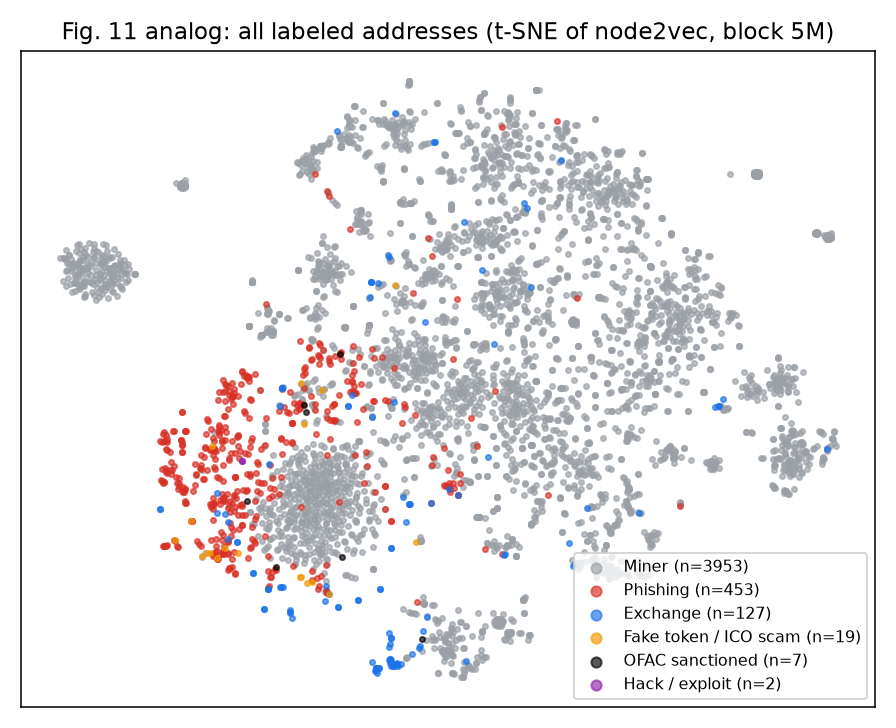
\includegraphics[width=0.66\textwidth]{figures/tsne_all}
\caption{Analog of the paper's Figure~11: t-SNE \cite{tsne} of dynamic node2vec embeddings (block 5\,M) for all labeled addresses. Phishing addresses (red) occupy a distinct region; miners (grey) cover most of the rest; exchanges (blue) are scattered.}
\label{fig:tsne_all}
\end{figure}
\begin{figure}[H]
\centering
\begin{subfigure}{0.48\textwidth}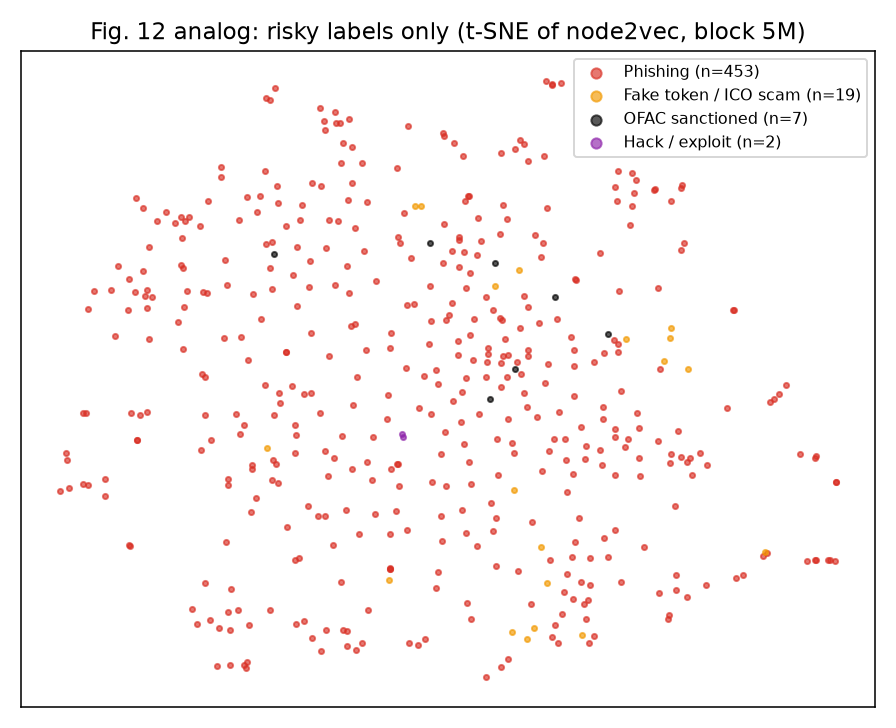
\includegraphics[width=\textwidth]{figures/tsne_risky}\caption{Risky labels only.}\end{subfigure}\hfill
\begin{subfigure}{0.48\textwidth}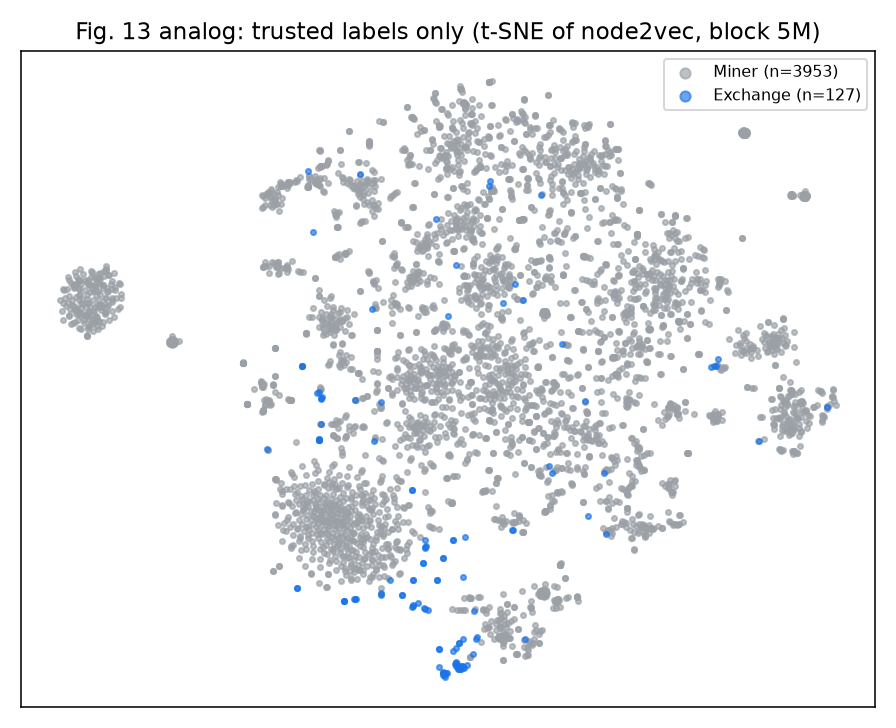
\includegraphics[width=\textwidth]{figures/tsne_trusted}\caption{Trusted labels only.}\end{subfigure}
\caption{Analogs of the paper's Figures~12 and~13, each projected separately.}
\label{fig:tsne_sub}
\end{figure}
``Visible clusters'' is a subjective criterion, so Table~\ref{tab:tsne} adds objective measures computed in the original 128-dimensional space, each next to a control with shuffled labels.
\begin{table}[H]
\centering\footnotesize\singlespacing
\begin{tabular}{l r cc cc c}
\toprule
 & $n$ & \multicolumn{2}{c}{silhouette (cosine)} & \multicolumn{2}{c}{5-NN accuracy} & majority\\
\cmidrule(lr){3-4}\cmidrule(lr){5-6}
 & & real & shuffled & real & shuffled & baseline\\
\midrule
Bad vs.\ good (all labeled) & 4,561 & 0.242 & -0.001 & 0.953 & 0.887 & 0.895\\
Six groups (Fig.~11 analog) & 4,559 & 0.011 & -0.070 & 0.938 & 0.857 & 0.867\\
Risky sub-types only (Fig.~12) & 479 & -0.148 & -0.068 & 0.948 & 0.946 & 0.942\\
Miners vs.\ exchanges (Fig.~13) & 4,080 & 0.457 & -0.014 & 0.979 & 0.969 & 0.969\\
\bottomrule
\end{tabular}
\caption{Cluster separation of the embeddings. Silhouette near 0 means no structure; 5-NN accuracy is 5-fold cross-validated and should be compared with the majority-class baseline.}
\label{tab:tsne}
\end{table}
The embedding separates the risk classes: bad versus good has a 5-NN accuracy of \TsneBadGoodKnn{} (balanced accuracy \TsneBadGoodBal) against a majority baseline of 0.895, and a silhouette of \TsneBadGoodSil{} (shuffled labels: about 0). Miners and exchanges also separate (silhouette 0.457). Finer sub-types of risky addresses (fake-token scams, hacks, OFAC) do not separate beyond the baseline, but these classes are tiny (19, 2 and 7 addresses) and noisily tagged, so no conclusion is possible for them.

\section{Scorecard and Analysis}
\label{sec:scorecard}
\begin{table}[H]
\centering\footnotesize\singlespacing
\begin{tabular}{p{3.7cm} p{3.0cm} p{5.3cm} p{1.8cm}}
\toprule
\textbf{Paper's claim} & \textbf{Paper} & \textbf{Our evidence} & \textbf{Verdict}\\
\midrule
Combining graph and behavioural features beats either alone (Table~II) & F$_1$ 0.851 vs.\ 0.738 / 0.718 & Gain +0.008 (A) / +0.004 (B), within noise; clean covered-only subset: 0.942 vs.\ 0.952 for behaviour alone & \vNo\\
Graph features beat behavioural features alone & 0.738 vs.\ 0.718 (gap 0.02, no CI) & Reversed: 0.871 (A), 0.753 (B) vs.\ 0.956 & \vNo\\
Dynamic node2vec beats propagation (Table~IV) & Gap 0.13--0.19 AUC at all checkpoints & Higher at all three checkpoints (+0.103, +0.037, +0.085 PR-AUC); clear only at 5.0\,M; full coverage vs.\ 79--89\% & \vPart\\
Best setting is 10 walks, length 10, $p=q=1$; more walks help (Table~III) & Best 0.814; walks 0.751 $\to$ 0.795 & Best \BestPRAUC{}; walks 0.865 $\to$ 0.929; $p,q$ effects within noise & \vOK\\
Propagation reaches about 78\% of addresses & 78\% (80--85\% of daily-active) & \CovA\% (A) and \CovB\% (B) on the whole graph; 98--100\% in our universe & \vPart\\
Embeddings show label clusters (Figs.\ 11--13) & Qualitative & Bad vs.\ good separable (5-NN \TsneBadGoodKnn{} vs.\ 0.895 baseline); sub-types not separable (tiny classes) & \vPart\\
Node2vec has high feature importance & Stated, not shown & 56.3\% (A), 46.7\% (B), biased by column count & \vPart\\
Scales to every address and updates incrementally & Deployed at 266\,M & Demonstrated on a 3\,M-node universe (checkpoint updates, bit-identical distributed walks); not tested at paper scale & untestable here\\
\bottomrule
\end{tabular}
\caption{Scorecard. ``Reproduced'' means the ordering or trend holds on our data, not that absolute numbers match.}
\label{tab:scorecard}
\end{table}

\subsection{Why do the headline claims differ?}
We rank explanations by how well our evidence supports them.
\begin{enumerate}
\item \textbf{Ceiling effect from an easy negative class (well supported).} Behavioural features alone reach F$_1$ 0.956, and with exchanges as the only negatives every feature set in variant A saturates at 0.98--0.99. When behaviour already separates the classes, there is little for graph embeddings to add. The paper's much lower behavioural score (0.718) leaves room for the complementary gain it reports.
\item \textbf{Different negative class (plausible).} Our negatives are miners and exchanges; the paper's include government addresses and, plausibly, a broader mix. We cannot verify this because its labels are private.
\item \textbf{Label noise and era mismatch (plausible, unmeasured).} Our labels are a 2022 snapshot of Etherscan tags applied to 2015--2018 activity, and labeled bad addresses may have been well known and structurally distinctive; the paper's labels come largely from curated internal sources plus undisclosed external ones.
\item \textbf{Scale (plausible).} Neighbourhood structure in a graph 11 times smaller and five years earlier may carry less signal. The coverage numbers show the geometry differs.
\item \textbf{Embedding quality at fixed budget (possible).} We trained one epoch at dimension 128 with unspecified skip-gram settings. Better-tuned embeddings could narrow the gap, but our sweep shows large gains from more walks, which suggests the node2vec features are not yet saturated; a longer training would be a cheap check.
\end{enumerate}

\subsection{What we can and cannot conclude}
We can conclude that the paper's \emph{engineering} claims hold up in direction: node2vec settings, the benefit of incremental embedding over propagation (with full coverage), and the practicality of a streaming, partitioned pipeline. We cannot confirm or refute its headline ablation, because our data differ in exactly the ways that would hide or reverse such an effect. We did \emph{not} find evidence that the paper is wrong; we found that the claim is fragile to the negative class.

\subsection{Threats to validity}
\begin{itemize}
\item \textbf{Single training run per method} in Tables~II and IV. The reported intervals reflect random train/test splits of fixed embeddings, not retraining variation, which we measured at about 0.01 PR-AUC. Part of the Table~IV gap could be training noise.
\item \textbf{Small bad class}, 481 addresses in total and 34 at the first checkpoint, makes some rows noisy.
\item \textbf{No external test set or temporal split.} Train and test addresses come from the same pool, as in the paper; a time-ordered split would be stricter.
\item \textbf{Label provenance} (Etherscan-derived) carries selection bias and a terms-of-use caveat.
\item \textbf{Multiple comparisons.} We inspected many configurations; the noise band guards against over-reading, but isolated differences should not be treated as findings.
\item \textbf{Unweighted snapshots, a 3\,M-node universe and a core that is a third of it} in Table~IV differ from the paper's larger core share relative to its universe.
\end{itemize}

\subsection{Inconsistencies and gaps found in the paper}
We list these neutrally; none changes our conclusions but each made reproduction harder.
\begin{enumerate}
\item The behavioural features are said to be ``defined in Table~1'', but Table~I is the data-source table; the feature list is never given.
\item The text says the hyperparameter AUC values are in ``Table~II''; they are in Table~III. Table~II is the feature-set comparison.
\item Table~III has blank cells (for example length~4, $p=0.25$ and $q=0.25$ rows).
\item The captions of Figures~8 and~9 appear swapped: Figure~8 is titled ``In-out Parameter (p)'' and Figure~9 ``Return parameter (q)''.
\item The graph size is given as about 266\,M addresses in the introduction and about 275\,M in the conclusion.
\item The dynamic-node2vec citation points to reference~[2], an unrelated paper on money laundering (dynnode2vec is reference~[11]), and the MapReduce citation points to reference~[3], also unrelated.
\item References [12] and [14] are the same paper listed with different years.
\item The hardware section mentions CPUs, PyTorch and ``GNN models'', although the system uses node2vec with gensim, and a footnote describes a V100 GPU.
\item The incremental step is described as ``daily'' while checkpoints are millions of blocks apart (about 830 daily steps from 10\,M to 16\,M); the actual step size is unclear.
\item The metric called ``AUC'' in Tables~III and~IV is not defined; Table~II's classification threshold is not stated; no uncertainty is reported anywhere.
\item Minor: the organisation paragraph refers to Section~6 for the conclusion (it is Section~V); ``Propogation'' is misspelled in an algorithm title.
\end{enumerate}

% =====================================================================================================
\section*{Part B: CryptoTrace}
\addcontentsline{toc}{section}{Part B: CryptoTrace}

\section{Evaluation Set-up}
\label{sec:evalsetup}
CryptoTrace was run on three cases (Table~\ref{tab:cases}). Two are documented hacks, taken from the textbook's case studies, whose published answers say where the funds went. The third is a real wallet that Etherscan users tagged as phishing; it has \emph{no} published answer, and it was selected from the public labels because its trace reaches exchange deposit addresses. That selection bias is disclosed in the application, in this report and in the case description. Each case was traced with three strategies: TTR-lite, Haircut taint and blind BFS (depth 2), with the default parameters of Table~\ref{tab:datamodel}.

\begin{table}[H]
\centering\small\singlespacing
\begin{tabular}{p{3.2cm} p{3.0cm} p{2.6cm} p{4.2cm}}
\toprule
\textbf{Case} & \textbf{Window} & \textbf{Funds leaving source} & \textbf{Published answer}\\
\midrule
Cryptopia exchange hack (May 2019) & 2019-05-14 to 2019-06-28 & 30\,766 ETH & EtherDelta within two hops; later Yobit.net and OKEx\\
KuCoin exchange hack (Sept.\ 2020) & 2020-09-25 to 2020-11-10 & 11\,533 ETH & About 13.8K ETH into the Tornado Cash 100 ETH pool\\
Phishing-labeled wallet (2018) & 2018-06-29 to 2018-08-13 & 2\,450 ETH & None (selected by us; label Fake\_Phishing1951)\\
\bottomrule
\end{tabular}
\caption{The three cases. Source addresses: Cryptopia \code{0xd4e79226\dots8d11}; KuCoin \code{0xeb31973e\dots8c23}; phishing \code{0x5457bb44\dots5b9b}.}
\label{tab:cases}
\end{table}

\section{Case 1: KuCoin Exchange Hack (September 2020)}
The hacker's wallet received ETH from KuCoin and moved most of it into Tornado Cash. TTR-lite reaches the Tornado Cash 100 ETH pool in two hops: 99.8\% of the funds, about 11\,511 ETH (Table~\ref{tab:dest_kucoin}). The evidence path has two transfers (Table~\ref{tab:path_kucoin}): 11\,500 ETH from the reported wallet to an intermediate address on 2020-10-23 at 07:40 UTC, then 100 ETH on to the pool at 08:06 UTC. The trace stops there because a mixer breaks the on-chain link; the destination is a high-confidence stop and the interface says that tracing cannot continue by this method. The published figure is about 13.8K ETH; ours is lower because of our window and the 0.01 ETH dust filter.

\gentable{gen/tab_dest_kucoin_2020.tex}{Destinations found for the KuCoin case (TTR-lite).}{tab:dest_kucoin}
\gentable{gen/tab_path_kucoin_2020.tex}{Evidence path to the Tornado Cash pool.}{tab:path_kucoin}
\gentable{gen/tab_rounds_kucoin_2020.tex}{Search rounds for the KuCoin case: accounts expanded, destinations absorbed and the share of funds still unexplained.}{tab:rounds_kucoin}

\shot{27_lab_kucoin_round1}{Trace Lab, KuCoin case, early in the search. The reported wallet and the first intermediate account appear; 85\% of the funds are still unexplained.}
\shot{28_lab_kucoin_final}{Trace Lab, KuCoin case, finished. The headline sentence states that 99.8\% of the traced funds reached Tornado Cash and that tracing stops at a mixer.}
\shot{29_lab_kucoin_mixer_expanded}{KuCoin case with the finding expanded: a high-confidence mixer stop, the two-transfer evidence path with transaction links, and the laundering pattern seen (one fast hop).}

\section{Case 2: Cryptopia Exchange Hack (May 2019)}
About 30.8K ETH was stolen from the Cryptopia exchange. TTR-lite follows 99.98\% of it (about 30\,760 ETH) to a single address in 500--1\,000 ETH batches, within six rounds; that address is the EtherDelta DEX contract (Table~\ref{tab:dest_cryptopia}). The curated label for EtherDelta is marked \emph{unverified on-chain}, so the finding carries medium confidence. The highest-value evidence path has five transfers (Table~\ref{tab:path_cryptopia}), and the shortest route to the contract is two hops. The share of unexplained funds falls more slowly than in the other cases (Table~\ref{tab:rounds_cryptopia}) because the funds move through a chain of intermediate accounts. The textbook reports that the funds later left through Yobit.net and OKEx; \emph{we do not reach these}, because they sit behind the DEX contract and the exit from a contract is an internal transfer, which the external-transfer data we use does not contain. We therefore record this case as one of three expected destinations reached (EtherDelta yes; Yobit.net and OKEx not reached) and list DEX pass-through as the first item of the pending work.

\gentable{gen/tab_dest_cryptopia_2019.tex}{Destinations found for the Cryptopia case (TTR-lite).}{tab:dest_cryptopia}
\gentable{gen/tab_path_cryptopia_2019.tex}{Evidence path to the EtherDelta contract (highest-value route).}{tab:path_cryptopia}
\gentable{gen/tab_rounds_cryptopia_2019.tex}{Search rounds for the Cryptopia case.}{tab:rounds_cryptopia}

\shot{30_lab_cryptopia_mid}{Trace Lab, Cryptopia case, mid-search (round 2 of 6): eight accounts, 72\% unexplained.}
\shot{31_lab_cryptopia_final}{Trace Lab, Cryptopia case, finished: 100\% of the traced funds (about 30\,760 ETH) reached the EtherDelta DEX contract; the note says that the way out is an internal transfer this prototype cannot yet follow.}
\shot{32_lab_cryptopia_dex_expanded}{Cryptopia finding expanded: medium confidence, ``labeled dex (curated; unverified on-chain)'', and the five-transfer evidence path. In total 18 transfers from the traced accounts entered the contract, about 9\,502 ETH of them visible within the window and the 200-transfer cap.}
\shot{33_lab_cryptopia_bfs_final}{Cryptopia traced by blind BFS: it also reaches the contract but attributes only 4.3\% of the funds to it, because it stops after two hops and splits shares uniformly.}

\section{Case 3: Phishing-Labeled Wallet (2018)}
\label{sec:phish}
This is the main demonstration case. A wallet that Etherscan users tagged as phishing sent about 2\,450 ETH between June and August 2018. TTR-lite finishes in five rounds touching 75 accounts and 1\,390 transfers (Table~\ref{tab:rounds_phish}); BigQuery was not queried at run time because the case was already cached. The results are:
\begin{itemize}
\item \textbf{90.9\% of the funds, about 2\,227 ETH, reached 29 distinct deposit addresses} that each forward their outflow to the labeled exchange wallet \emph{ShapeShift 3} (the sweep rule), within two hops. These are inferred deposit addresses with medium confidence (Table~\ref{tab:dest_phish}, Figure~\ref{fig:deposit_share}).
\item \textbf{5.2\%, about 128 ETH, reached two unlabeled high-activity services} (one with 10\,512 and one with 17\,869 transfers in the window), where the trace stops with low confidence and a manual-review flag (Table~\ref{tab:hubs}).
\item The funds first move in one transfer of 2\,198 ETH to an intermediate account on 2018-07-11, which splits them mainly into 100 ETH pieces. The highest-value evidence path to a deposit address has three transfers (Table~\ref{tab:path_phish_top}): 2\,198 ETH, then 101 ETH, then 10.2 ETH, ending at the deposit address \code{0x5ea511\dots04f1} on 2018-07-19.
\item The typology engine tags 26 accounts as zero-out (forwarding almost everything within a day) and 27 as fast hops (Table~\ref{tab:tags}).
\end{itemize}

\gentable{gen/tab_dest_phishing_2018.tex}{Destinations found for the phishing case (TTR-lite). Twenty-nine deposit addresses are grouped into one finding.}{tab:dest_phish}
\gentable{gen/tab_rounds_phishing_2018.tex}{Search rounds for the phishing case.}{tab:rounds_phish}
\gentable{gen/tab_hubs.tex}{The two unlabeled high-activity services where the phishing trace stops.}{tab:hubs}

\begin{figure}[H]
\centering
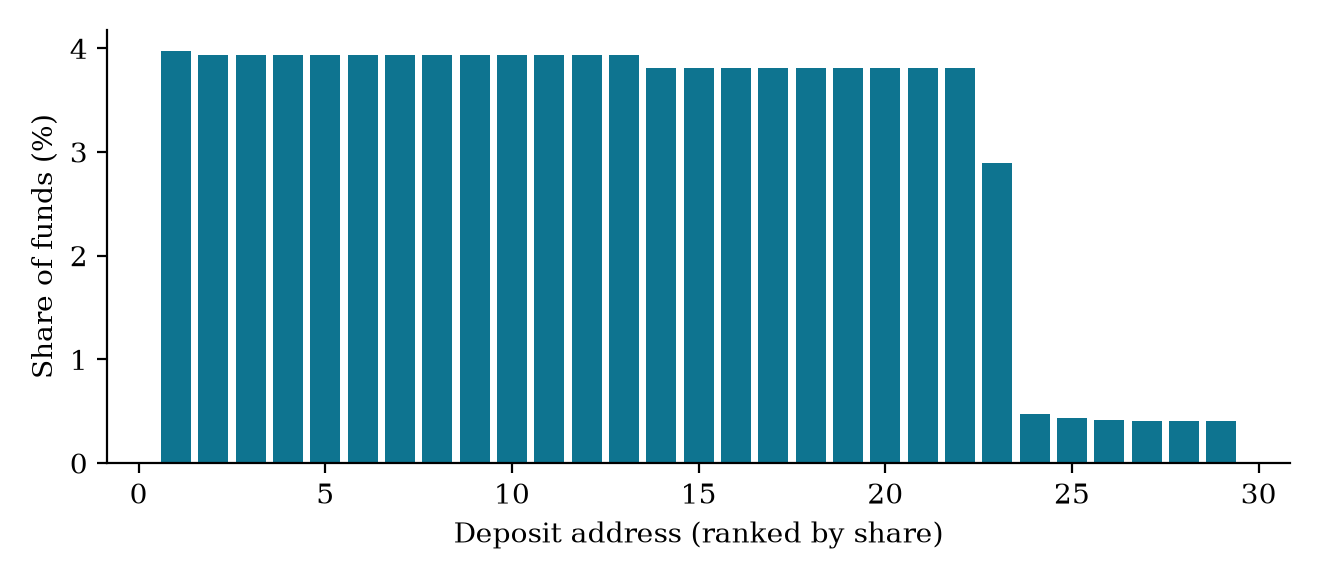
\includegraphics[width=0.9\textwidth]{figs/deposit_share.png}
\caption{Share of the funds reaching each of the 29 deposit addresses, ranked. Twenty-two addresses receive about 3.8--4.0\% each, which matches the splitting of the funds into near-equal pieces; the last six receive about 0.4\% each.}
\label{fig:deposit_share}
\end{figure}

\begin{figure}[H]
\centering
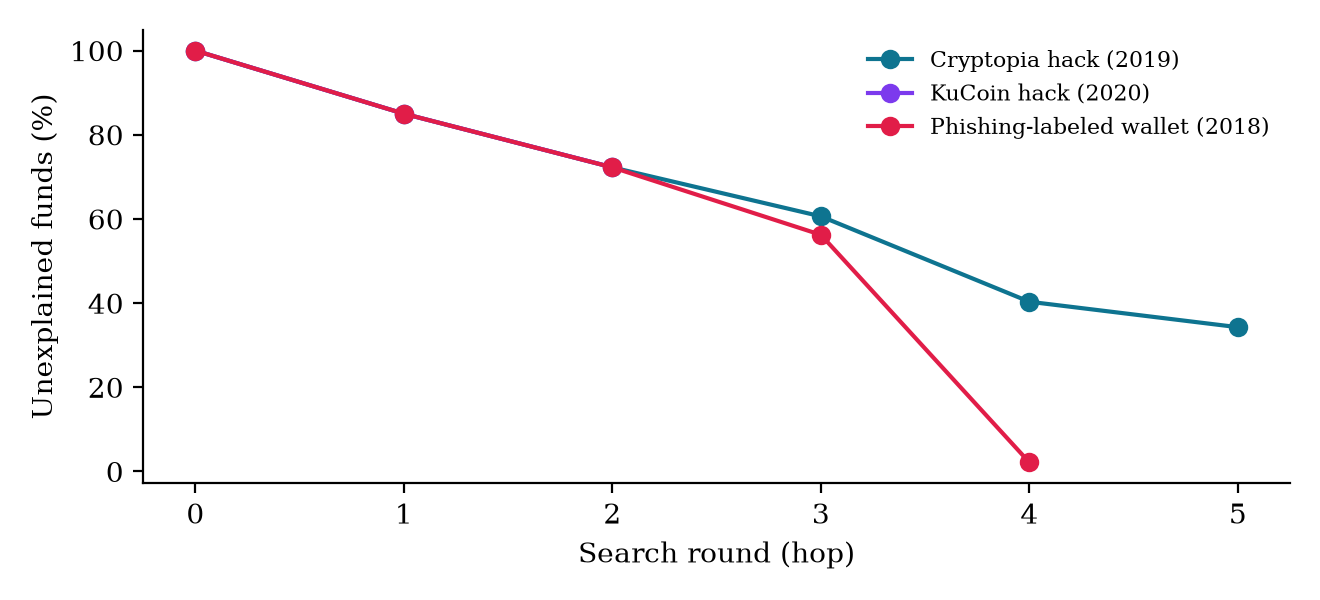
\includegraphics[width=0.9\textwidth]{figs/residual_decay.png}
\caption{Unexplained funds after each search round for the three cases. The phishing case drops from 56\% to 2\% in round 4, when the deposit addresses are reached; the Cryptopia case declines more slowly because the funds pass through a chain of accounts.}
\label{fig:residual_decay}
\end{figure}

\subsection{Stepping through the search}
Figures~\ref{fig:13_lab_phishing_start} to~\ref{fig:17_lab_phishing_final} show the same trace at successive rounds, exactly as the application plays it. At round 0 only the reported wallet exists. In round 1 the search fetches its neighbourhood (one cached lookup) and finds the first recipient. By round 2 the 100 ETH pieces appear. In round 3 the frontier grows to 32 accounts and the first deposit addresses are absorbed, and in round 4 the remaining funds are explained and 2\% remain unexplained, at which point the search ends.

\shot{13_lab_phishing_start}{Phishing case, round 0: only the reported wallet. The result column already shows the stored finding; the data-layer counter reads 0 queries, 0 cached.}
\shot{14_lab_phishing_round1}{Round 1: four accounts and four transfers; 85\% of the funds are unexplained; one cached lookup.}
\shot{15_lab_phishing_round2}{Round 2: 29 accounts and 29 transfers; 72\% unexplained. The hub that splits the funds appears.}
\shot{16_lab_phishing_round3}{Round 3: 44 accounts; 56\% unexplained; 37 cached lookups. The first deposit addresses are absorbed (teal rings).}
\shot{17_lab_phishing_final}{Round 4: 2\% unexplained, 63 cached lookups, no queries. The top finding is highlighted automatically when playback ends, and its deposit address is labeled on the canvas.}

\subsection{Reading the finding}
The finding card (Figure~\ref{fig:18_lab_phishing_group_expanded}) states the entity (ShapeShift 3), the number of addresses (29), the share and amount (90.9\%, about 2\,227 ETH), the confidence (medium), the type (exchange deposit, inferred) and the rule that produced it (``forwards 100\% of its outflow to ShapeShift 3 within 48 h''). Below it is the list of addresses to ask the exchange to freeze, with each address's share and amount, and the evidence path to the largest of them (Figure~\ref{fig:19_lab_phishing_paths}), each transfer with its amount, time and a link to the transaction on a public block explorer.

\shot{18_lab_phishing_group_expanded}{The grouped finding expanded: ShapeShift 3, 29 addresses, medium confidence, the sweep rule, and the addresses to ask the exchange to freeze.}
\shot{19_lab_phishing_paths}{Evidence path to the largest deposit address (three transfers with timestamps and transaction links), and a statement of how many transfers in total entered these addresses (287, about 2\,308 ETH).}

\gentable{gen/tab_path_phishing_2018.tex}{Evidence path recorded in the case file for the first service account on the phishing trace (the hub reached through the 100 ETH piece).}{tab:path_phish_hub}
\begin{table}[H]
\centering\small\singlespacing
\begin{tabular}{r p{2.9cm} p{2.9cm} r p{2.5cm}}
\toprule
\textbf{\#} & \textbf{From} & \textbf{To} & \textbf{ETH} & \textbf{Time (UTC)}\\\midrule
1 & \texttt{0x5457bb..7c5b9b} & \texttt{0x5979e2..0c6f14} & 2\,198.39 & 2018-07-11 21:05\\
\multicolumn{5}{l}{\quad tx: \texttt{\scriptsize 0x445f791d730719386f01a56ca2d5dd78d85604a1581d0f636116d4c585122485}}\\
2 & \texttt{0x5979e2..0c6f14} & \texttt{0x76fc36..f646a0} & 101.14 & 2018-07-19 13:32\\
\multicolumn{5}{l}{\quad tx: \texttt{\scriptsize 0x9d81bd959bee5cf670e0f3b113c77abd41714dc6567a8e2cbc7da2922c364ad1}}\\
3 & \texttt{0x76fc36..f646a0} & \texttt{0x5ea511..04f1} & 10.20 & 2018-07-19 14:19\\
\multicolumn{5}{l}{\quad tx: \texttt{\scriptsize 0x027926853601d26e17fecfd23ac3206ff8e79b4934a6cbb5399534d63eb8a904}}\\
\bottomrule\end{tabular}
\caption{Evidence path to the largest deposit address (3.98\% of the funds), from the case file.}
\label{tab:path_phish_top}
\end{table}

\subsection{Inside the engine, and a single account}
The \emph{Inside the engine} tab (Figure~\ref{fig:20_lab_phishing_engine_tab}) narrates what the engine did in the current round: the frontier size, the weights of the highest-residual accounts, the unexplained funds per round as a small chart, and the list of stops with the rule that triggered each. The \emph{Account} tab (Figure~\ref{fig:21_lab_phishing_account_tab}) describes a clicked account: its address with a link to the explorer, role, label, share of funds, hops from the source, time of first funds, transfers in and out within the window, and its rank.

\shot{20_lab_phishing_engine_tab}{The \emph{Inside the engine} tab: each stop is listed with the sweep rule that triggered it.}
\shot{21_lab_phishing_account_tab}{The \emph{Account} tab for the deposit address \code{0x5ea511\dots04f1}: role exchange deposit (inferred), 3.98\% of funds, three hops, first funds 2018-07-19 13:44 UTC, 12 transfers in and 2 out.}
\shot{22_lab_parameters_panel}{The result column scrolled to show the second finding (two unlabeled high-activity services, low confidence), the laundering patterns seen (zero-out 26, fast hop 27) and the limits of the prototype; the control column shows the parameter sliders and the Run trace button.}

\gentable{gen/tab_tags.tex}{Laundering-pattern tags per case (number of accounts tagged, TTR-lite).}{tab:tags}

\section{Comparison of the Three Strategies}
Table~\ref{tab:runs} lists every run. On the two documented hacks all three strategies reach the published destination, but with different effort and different attribution of the funds. On the phishing case the strategies separate: TTR-lite and Haircut taint each reach 31 destinations (29 deposit addresses and two hubs), while blind depth-2 BFS reaches none, because the funds only arrive at deposit addresses after the third hop and the BFS stops after the second.

\gentable{gen/tab_runs.tex}{All nine runs: rounds, accounts in the result graph, transfers considered, depth, destinations reached and the top destination with its share.}{tab:runs}

\begin{figure}[H]
\centering
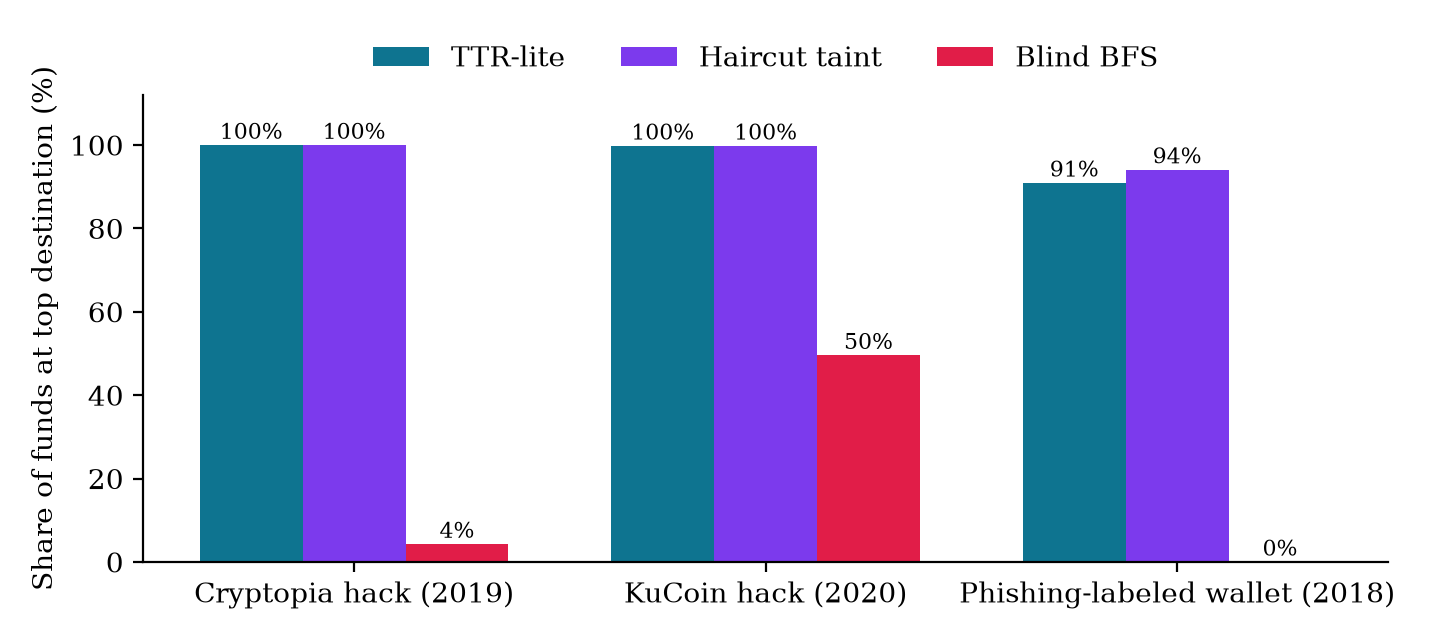
\includegraphics[width=0.95\textwidth]{figs/share_by_engine.png}
\caption{Share of the funds attributed to the top destination, by case and strategy. BFS attributes only 4\% (Cryptopia) and 50\% (KuCoin) of the funds to the correct destination and 0\% on the phishing case.}
\label{fig:share_by_engine}
\end{figure}
\begin{figure}[H]
\centering
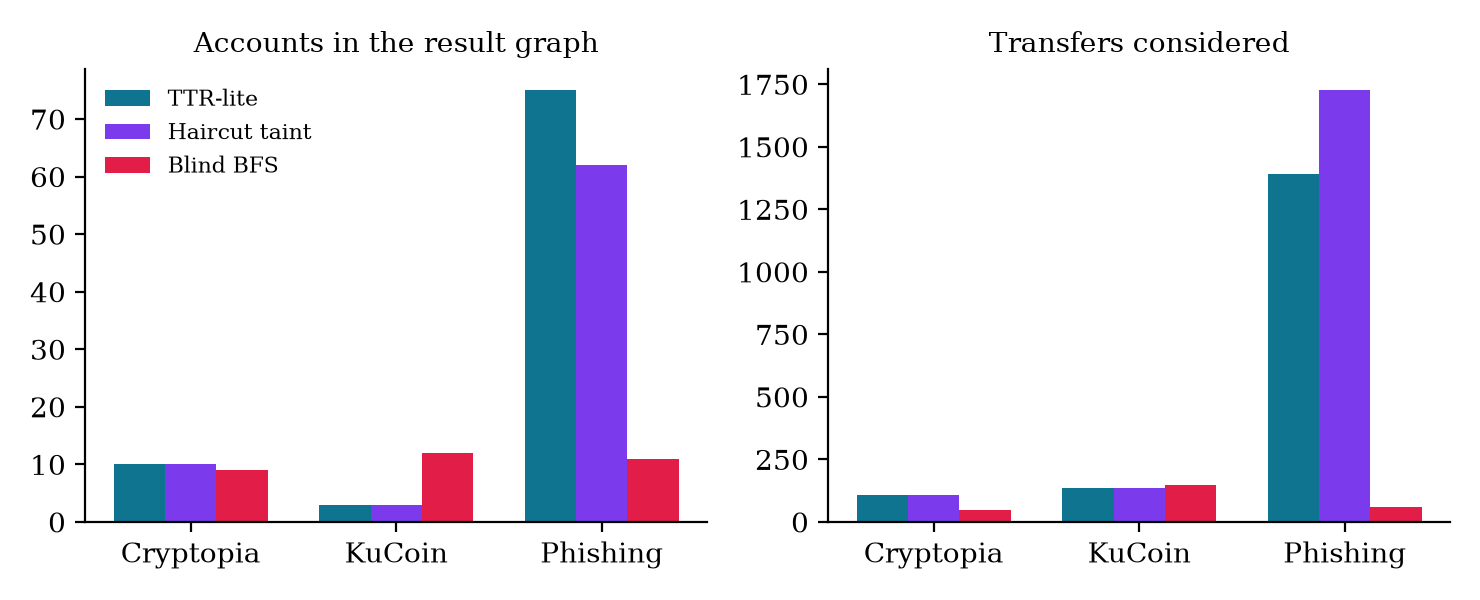
\includegraphics[width=0.98\textwidth]{figs/effort_by_engine.png}
\caption{Effort by strategy: accounts in the result graph (left) and transfers considered (right).}
\label{fig:effort}
\end{figure}

\paragraph{Observations.}
\begin{itemize}
\item \emph{Ranked and taint searches agree closely.} On KuCoin and Cryptopia their results are identical; on the phishing case they differ slightly (90.9\% against 94.1\% attributed to ShapeShift 3; 75 against 62 accounts; five against seven rounds). TTR-lite also follows a small share backwards, which adds upstream accounts to the graph.
\item \emph{BFS fails in two different ways.} It reaches no destination at all on the phishing case, and on the two hacks it reaches the right destination but attributes only a fraction of the funds to it (4.3\% and 49.6\%), since it spreads shares uniformly across every neighbour.
\item \emph{BFS is not reliably cheaper.} On the Cryptopia and phishing cases it considers far fewer transfers than the ranked search (48 against 106, and 59 against 1\,390), which is exactly why it stops short; on KuCoin it considers slightly more (146 against 135) and returns more accounts (12 against 3) for an investigator to review.
\item \emph{This separation matches the published benchmark in kind.} The textbook's 20-case table (Table~\ref{tab:bookbench}) shows blind BFS reviewing about 52\,500 accounts for 77\% recall and the ranked search about 870 for 92\%. Our three cases are too few to say anything about numbers, only about direction.
\end{itemize}

\shot{24_lab_phishing_haircut_final}{Phishing case with the Haircut strategy: the same destination with 94.1\% of the funds, seven rounds.}
\shot{25_lab_phishing_bfs_final}{Phishing case with blind BFS: the search ends after two hops without reaching any labeled destination, and the interface explains why.}

\section{What-If Re-Runs at Zero Cost}
Because every neighbourhood is cached, parameters can be changed and the trace re-run at once with no BigQuery cost. Figure~\ref{fig:26_lab_whatif_3rounds} shows the phishing case re-run with the maximum number of rounds lowered to three. The search stops at the hop limit and the interface warns that unexplored flows remain; 56\% of the funds are still unexplained, only 5 of the 29 deposit addresses have been reached (about 4.5\% of the funds, roughly 108 ETH), the unlabeled hub holds 4.1\% (about 100 ETH), and the data-layer counter shows 37 cached lookups and no queries. This is how a presenter can show the algorithm responding to its settings without waiting.

\shot{26_lab_whatif_3rounds}{What-if re-run with the round limit lowered to 3: the search stops early, a warning says unexplored flows remain, and the unexplained share stays at 56\%.}

\section{BigQuery Cost}
Table~\ref{tab:cost} and Figure~\ref{fig:bq_cost} summarise the cost of first fetches. A per-hop query returns only the largest transfers per address, but BigQuery bills by the partitions scanned for the time window, so the cost depends on the window and not on the number of addresses in a chunk. Each case therefore cost cents, and all later runs were free.

\begin{table}[H]
\centering\small\singlespacing
\begin{tabular}{p{5.2cm} r r}
\toprule
\textbf{Item} & \textbf{Scanned (GiB)} & \textbf{List-price cost (USD)}\\
\midrule
Reproduction extraction (blocks 0--5\,M, Tier S) & 48.6 & about 0.30\\
Cryptopia case, first fetch & 9.51 & about 0.06\\
KuCoin case, first fetch & 3.87 & about 0.02\\
Phishing case, first fetch & 19.90 & about 0.12\\
Exploration query used to find the phishing example & 29.9 & about 0.18\\
\bottomrule
\end{tabular}
\caption{BigQuery scanning at an assumed list price of \$6.25 per TiB (to be checked against current pricing; the first TiB each month is free). Total for the tracing prototype, including other exploration, is roughly \$0.6.}
\label{tab:cost}
\end{table}
\begin{figure}[H]
\centering
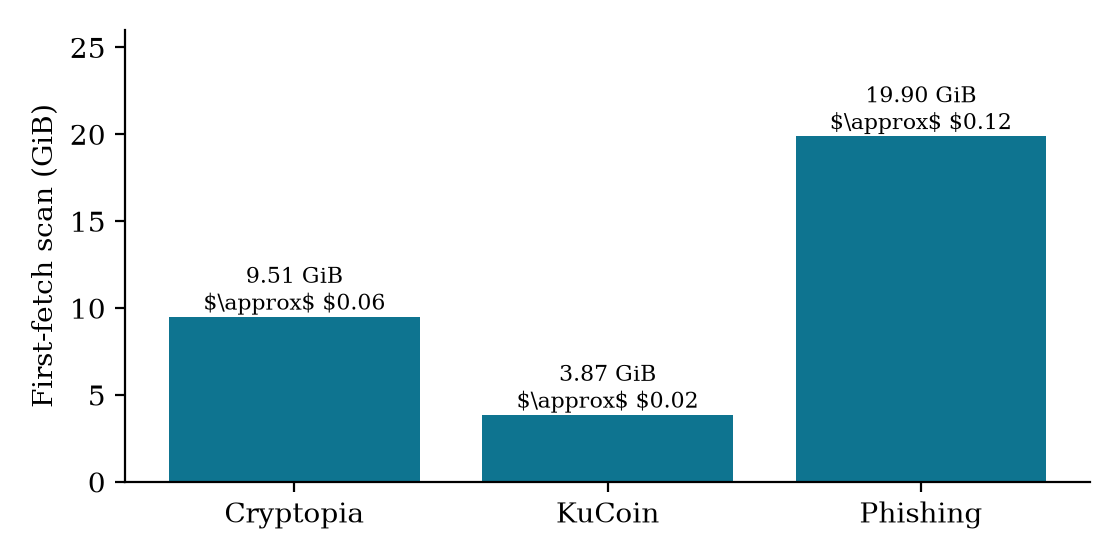
\includegraphics[width=0.7\textwidth]{figs/bq_cost.png}
\caption{First-fetch scan size and approximate cost per case.}
\label{fig:bq_cost}
\end{figure}

\section{A Walk through Every Screen}
\label{sec:screens}
This section shows every screen of the application. All screenshots were taken by a script (\code{scripts/ct\_screenshots.mjs}) that drives a real browser against the running application at a 1440$\times$900 viewport at 1.5$\times$ resolution, selecting the case, strategy and search round explicitly for each image. Full-page captures are in Appendix~\ref{app:screens}.

\subsection{Overview}
The Overview page (Figure~\ref{fig:01_overview_top}) states the problem in one sentence and gives four headline figures: 100\% of the Cryptopia funds followed to the EtherDelta DEX in six rounds; 99.8\% of the KuCoin funds followed into the Tornado Cash pool in three rounds, where tracing correctly stops; the cost of the first full Cryptopia trace (about \$0.06); and ``29 $\to$ 1'', the number of deposit addresses traced from one phishing-labeled wallet into a single exchange. Below are the four steps of a trace (report a wallet, follow the money, stop at a service, hand over evidence) and the three cases, each with its headline result, number of rounds, accounts in the graph and first-fetch size. A closing box states what the prototype is and is not.

\shot{01_overview_top}{Overview page: headline figures, how a trace works, and the cases.}
\shotw{44_overview_tablet}{The Overview page at tablet width (820 px): the cards reflow into two columns.}{0.5}

\subsection{System}
The System page (Figure~\ref{fig:03_system_idle}) draws the architecture of Chapter~\ref{ch:design} from the module data: five columns (intake, data layer, engines, output, evaluation), each module with its status (live, partial or planned), a switch to hide the planned modules, and dashed arrows for data flow. Clicking a module opens its details: what it does, what is live and what is pending, which problem-statement requirements it serves. The button \emph{Play a trace through the system} replays a real trace through the modules (Figures~\ref{fig:05_system_playing} and~\ref{fig:06_system_playing_late}): the intake opens the case, the adapter fetches, the cache reports its first-fetch size, the tracing engine reports each round and the share of funds still unexplained, the attribution engine states where it stops, the typology engine counts the patterns, and the case file and report are written. A log on the page narrates each step with the numbers of the case.

\shot{03_system_idle}{System page at rest: status badges, the planned modules shown dashed, and the data-flow arrows.}
\shot{05_system_playing}{System page while a trace plays through the modules (the tracing engine is lit).}
\shot{06_system_playing_late}{Later in the same playback: the investigator report is lit.}

\subsection{Trace Lab}
The Trace Lab is the centre of the application and has been shown above case by case. Its three columns are the \emph{controls} (demo guide, case picker with the case's story, strategy buttons with a one-line description of each strategy, parameter sliders for $\alpha$, $\beta$, $\epsilon$, maximum rounds and hub threshold, a time-respecting switch and a Run button), the \emph{graph} with a heads-up display (round, accounts, transfers, unexplained share, data layer), a legend and a playback bar (back, play or replay, forward, scrubber, speed, fit), and the \emph{result column} with the tabs Findings, Inside the engine and Account. The case picker can be switched to \emph{Any wallet} (Figures~\ref{fig:34_lab_anywallet_empty} and~\ref{fig:35_lab_anywallet_cache_miss}): the user enters an address and dates; live BigQuery access is a switch that is off unless the server was started with credentials, so an address that was never fetched ends with a clear message instead of a bill.

\shot{34_lab_anywallet_empty}{The \emph{Any wallet} mode of the case picker (the previous result is still shown until a new run starts).}
\shot{35_lab_anywallet_cache_miss}{A custom address that was never fetched: ``1 address(es) are not cached for this window; enable live BigQuery to fetch them''. Nothing is billed.}
\shotw{23_lab_phishing_1280x720}{The Trace Lab at 1280$\times$720, the projector size: the three columns fit without scrolling the page.}{0.85}

\subsection{Compare}
The Compare page (Figures~\ref{fig:36_compare_phishing}--\ref{fig:38_compare_cryptopia}) has one tab per case and a table with one row per strategy: expected destinations found (for cases with a published answer, with a tick or cross per expected name; ``no published answer'' otherwise), destinations reached, accounts to audit, transfers considered, maximum depth, rounds and run time. Three bar charts show accounts to audit, transfers considered and deepest hop. A box headed ``Reading this honestly'' adapts to the case: on the phishing case it says that the strategies separate and that the case is an illustration, not a measured accuracy; on the other two it says that all strategies end at the same destination and differ in effort. At the bottom is the textbook's published 20-case table (Table~\ref{tab:bookbench}).

\shot{36_compare_phishing}{Compare, phishing case: TTR-lite and Haircut reach 31 destinations, BFS reaches 0; no published answer to score against.}
\shot{37_compare_kucoin}{Compare, KuCoin: all three strategies find the Tornado Cash pool (one of one expected destination) with different effort.}
\shot{38_compare_cryptopia}{Compare, Cryptopia: EtherDelta found by all three strategies, Yobit.net and OKEx not found by any (one of three).}

\subsection{Gaps}
The Gaps page (Figure~\ref{fig:40_gaps_top}) presents eight research gaps in plain words, each with the gap, the evidence and what this prototype does about it, followed by a roadmap of what is built, partial and planned, and the list of requirements from the problem statement that remain to be clarified, including the SAHYOG and NCRP integration for which no specification was available.

\shot{40_gaps_top}{Gaps page: research gaps with evidence and the prototype's response.}

\subsection{Report}
The Report page (Figures~\ref{fig:42_report_top}) turns the current trace into a printable investigator report on a white page: the case (reported wallet, window, funds leaving), a summary sentence, the destinations reached, the addresses to ask the exchange to freeze, the evidence paths with transaction hashes, the laundering patterns observed, and the method, limits and confidence. A button prints the page or saves it as a PDF.

\shot{42_report_top}{Report page (top): case, summary, destinations and the addresses to freeze.}

\section{What Was Improved over the Baseline, and What Was Not}
\label{sec:improvements}
Table~\ref{tab:improve} states the differences between the baseline and the extension in concrete terms.

\begin{table}[H]
\centering\small\singlespacing
\begin{tabular}{p{2.5cm} p{5.0cm} p{5.3cm}}
\toprule
\textbf{Aspect} & \textbf{RiskSEA (baseline)} & \textbf{CryptoTrace (extension)}\\
\midrule
Task & Score each wallet in $[0,1]$ & Trace funds from a reported wallet to the receiving entity\\
Graph & One global, count-weighted graph (24\,M addresses in our reproduction) & Built on demand around the case; keeps direction, amount, time and transaction hash\\
Algorithm & node2vec embeddings and a random forest; training needed & Local ranked propagation; no training; 75 accounts touched on the phishing case\\
Direction and time & Undirected, untimed walks & Directed, time-respecting, value-weighted\\
Attribution & None & Stops at exchanges, mixers, DEX, hubs; infers exchange deposit addresses\\
Evidence & A probability & Hash-level transaction paths and readable pattern tags\\
Data access & Bulk extraction (48.6\,GiB) & One query per hop; cents per case; free re-runs\\
Evaluation & F$_1$ and PR-AUC & Destinations reached and accounts to audit, over three strategies\\
Delivery & Scripts and reports & API with live events and an interactive application\\
\bottomrule
\end{tabular}
\caption{Baseline versus extension.}
\label{tab:improve}
\end{table}

\paragraph{What was not improved.} We make no claim of a better score on RiskSEA's own task: our reproduction did not confirm that graph embeddings beat behavioural features on our data. The extension solves a different problem and is evaluated on a different criterion. The RiskSEA reproduction is not yet wired into CryptoTrace; it is the planned risk-model module.

\section{Limits of the Results}
\begin{itemize}
\item \textbf{Three cases are a smoke test.} We have not run the 20-case benchmark; its case files were not available to us. Nothing here measures accuracy.
\item \textbf{One case has no published answer.} It was selected because its trace reaches exchange deposits, so it shows the method, not the hit rate of the method on arbitrary wallets.
\item \textbf{Deposit-address attribution is inferred.} The sweep rule gives a strong lead; the exchange must confirm it. The ShapeShift 3 label itself comes from a public, Etherscan-derived list.
\item \textbf{ETH external transfers only.} Funds that move through contracts, ERC-20 tokens, stablecoins or other chains are not followed; the Cryptopia trace stops at a contract for this reason.
\item \textbf{Coverage caps.} Only the 200 largest transfers per address and direction, and transfers of at least 0.01 ETH, are considered; the numbers of transfers entering a destination in the findings are therefore lower bounds.
\item \textbf{Near-real-time at best.} The public dataset lags the chain.
\end{itemize}
